\subsection{Discrete Time Compounding}
We work in a finite-horizon discrete-time model indexed by $\left\{0,1,\dots,N\right\}$
\begin{center}
	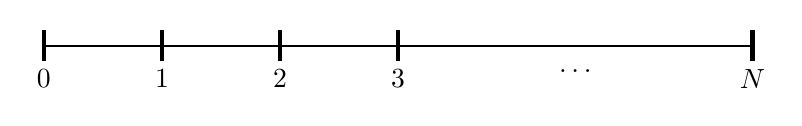
\begin{tikzpicture}[x=1.5cm, y=1cm]
		% Continuous horizontal timeline
		\draw[thick] (0,0) -- (6,0);

		% Ticks and Labels for 0, 1, 2, 3
		\foreach \x in {0, 1, 2, 3} {
				\draw[ultra thick] (\x, -0.2) -- (\x, 0.2);
				\node[below=5pt] at (\x, 0) {$\x$};
			}

		% Ellipsis label in the gap
		\node[below=5pt] at (4.5, 0) {$\dots$};

		% Final N tick and label
		\draw[ultra thick] (6, -0.2) -- (6, 0.2);
		\node[below=5pt] at (6, 0) {$N$};
	\end{tikzpicture}
\end{center}
We invest a cash flow $C$ each year in an investment plan that carries a constant interest rate $r$. At the end of the $N$-th year, the value of the amount $C$ invested at the beginning of year $k = 1, 2, \dots, N$ has turned into $C(1+r)^{N-k+1}$ and the total value of the plan $V_N$ at the end of the $N$-th year becomes
\begin{align}
	V_N & = C \sum_{k=1}^{N} (1+r)^{N-k+1} \nonumber \\
	    & = C \sum_{k=1}^{N} (1+r)^k \nonumber       \\
	    & = C(1+r) \frac{(1+r)^N - 1}{r},
\end{align}
hence the duration $N$ of the plan satisfies
\begin{equation}
	N+1 = \frac{1}{\log(1+r)} \log \left( 1+r + \frac{r V_N}{C} \right).
\end{equation}
\noindent At time $t=0$ one borrows an amount $L$ over a period of $N$ years at the constant interest rate $r$ per year.

\begin{prop}{Constant Repayment}{Repayment}
	Assuming the loan is fully amortized at the beginning of year $N+1$, the constant annual repayment $C$ is uniquely determined by
	\begin{equation}
		C = \frac{r(1+r)^N L}{(1+r)^N - 1} = \frac{r}{1 - (1+r)^{-N}} L.
	\end{equation}
\end{prop}
\begin{proof}
	Let $L_k$ denote the outstanding principal balance at the beginning of year $k$, with $L_1 = L$. The evolution of the debt is governed by the linear recurrence relation
	\begin{equation}
		L_{k+1} = (1+r)L_k - C, \quad \forall k \ge 1.
	\end{equation}
	Iteratively expanding this relation yields the value of the debt at the start of any arbitrary year $k$
	\begin{align}
		L_k & = (1+r)^{k-1}L_1 - C \sum_{j=0}^{k-2} (1+r)^j \nonumber                 \\
		    & = (1+r)^{k-1}L - C \frac{(1+r)^{k-1} - 1}{r}. \label{eq:BalanceGeneral}
	\end{align}
	The amortization condition requires that the debt is extinguished at the horizon $N$, such that $L_{N+1} = 0$. Substituting $k=N+1$ into \cref{eq:BalanceGeneral} implies
	\[
		0 = (1+r)^N L - C \frac{(1+r)^N - 1}{r}.
	\]
	Rearranging for $C$ yields the result in \ref{prop:Repayment}. Furthermore, substituting this expression for $C$ back into \cref{eq:BalanceGeneral} provides the closed-form outstanding balance
	\begin{equation}
		L_k = \frac{C}{r} \left[ 1 - (1+r)^{k-1-N} \right] \equiv \frac{C - (1+r)^{k-1}(C - rL)}{r}.
	\end{equation}
\end{proof}
\noindent Rearranging the result in \ref{prop:Repayment} yields the annuity factor
\begin{equation}
	\frac{L}{C} = \frac{1 - (1+r)^{-N}}{r},
\end{equation}
and solving for the duration $N$ implies
\begin{equation}
	N = \frac{1}{\log(1+r)} \log \left( \frac{C}{C - rL} \right) = - \frac{\log(1 - \frac{rL}{C})}{\log(1+r)}.
\end{equation}
\begin{xtip}
	For $N$ to be finite, we require the condition $C > rL$. This means the annual repayment must exceed the interest accrued on the initial principal; otherwise, the principal balance will never decrease.
\end{xtip}

\begin{prop}{Repayment Decomposition}{Decomposition}
	The $k$-th repayment $C$ decomposes into an interest component $rL_k$ and a principal repayment component $C - rL_k$ given by
	\begin{align}
		rL_k     & = C \left( 1 - \frac{1}{(1+r)^{N-k+1}} \right) = C r \sum_{l=1}^{N-k+1} (1+r)^{-l} \label{eq:InterestComp} \\
		C - rL_k & = \frac{C}{(1+r)^{N-k+1}}, \quad k=1, 2, \dots, N. \label{eq:PrincipalComp}
	\end{align}
\end{prop}

\begin{proof}
	Recall from the proof of \ref{prop:Repayment} that the outstanding balance $L_k$ represents the present value of the remaining $N-k+1$ payments. We express $L_k$ as
	\begin{equation}
		L_k = \frac{C}{r} \left[ 1 - (1+r)^{-(N-k+1)} \right].
	\end{equation}
	Multiplying by $r$ immediately yields the interest component in \cref{eq:InterestComp}. Consequently, the principal repayment is determined by the residual
	\begin{align}
		C - rL_k & = C - C \left[ 1 - (1+r)^{-(N-k+1)} \right] \nonumber \\
		         & = C (1+r)^{-(N-k+1)},
	\end{align}
	which corresponds to \cref{eq:PrincipalComp}.
\end{proof}

\noindent We verify that the sum of discounted payments at rate $r$ recovers the initial loan amount
\begin{equation}
	\sum_{l=1}^{N} \frac{C}{(1+r)^l} = C \frac{1 - (1+r)^{-N}}{r} = L.
\end{equation}
In particular, the first interest repayment satisfies
\begin{equation}
	rL_1 = C r \sum_{l=1}^{N} \frac{1}{(1+r)^l} = C \left( 1 - (1+r)^{-N} \right),
\end{equation}
and the first principal repayment is
\begin{equation}
	C - rL = \frac{C}{(1+r)^N}.
\end{equation}

\subsection{The Model}
\begin{defn}{num\'{e}raire}{Numeraire}
	A \emph{num\'{e}raire} is a price process $(X(t))_{t=0}^T$ (a sequence of random variables), which is strictly positive for all $t \in \{0, 1, \dots, T\}$.
\end{defn}

For the standard approach the risk-free bank account process is used as num\'{e}raire. In some applications, however, it is more convenient to use a security other than the bank account and we therefore just use $S_0$ without loss of generality.

\begin{defn}{Value of the Portfolio}{ValueOfThePortfolio}
	The value of the portfolio at time $t$ is the scalar product
	\begin{equation*}
		V_\varphi(t) = \varphi(t) \cdot S(t) \coloneqq \sum_{i=0}^d \varphi_i(t)S_i(t), \quad (t=1, 2, \dots, T) \text{ and } V_\varphi(0) = \varphi(1) \cdot S(0).
	\end{equation*}
	The process $V_\varphi(t, \omega)$ is called the \emph{wealth} or \emph{value process} of the trading strategy $\varphi$.
\end{defn}

The initial wealth $V_\varphi(0)$ is called the \emph{initial investment} or \emph{endowment} of the investor.

Now $\varphi(t) \cdot S(t-1)$ reflects the market value of the portfolio just after it has been established at time $t-1$, whereas $\varphi(t) \cdot S(t)$ is the value just after time $t$ prices are observed, but before changes are made in the portfolio. Hence
\begin{equation*}
	\varphi(t) \cdot (S(t) - S(t-1)) = \varphi(t) \cdot \Delta S(t)
\end{equation*}
is the change in the market value due to changes in security prices which occur between time $t-1$ and $t$. This motivates the following definition.

\begin{defn}{Gains Process}{GainsProcess}
	The \emph{gains process} $G_\varphi$ of a trading strategy $\varphi$ is given by
	\begin{equation*}
		G_\varphi(t) \coloneqq \sum_{\tau=1}^t \varphi(\tau) \cdot (S(\tau) - S(\tau-1)) = \sum_{\tau=1}^t \varphi(\tau) \cdot \Delta S(\tau), \quad (t=1, 2, \dots, T).
	\end{equation*}
\end{defn}

Define $\tilde{S}(t) = (1, \beta(t)S_1(t), \dots, \beta(t)S_d(t))'$, the vector of discounted prices, and consider the \emph{discounted value process}
\begin{equation*}
	\tilde{V}_\varphi(t) = \beta(t)(\varphi(t) \cdot S(t)) = \varphi(t) \cdot \tilde{S}(t), \quad (t=1, 2, \dots, T)
\end{equation*}
and the \emph{discounted gains process}
\begin{equation*}
	\tilde{G}_\varphi(t) \coloneqq \sum_{\tau=1}^t \varphi(\tau) \cdot (\tilde{S}(\tau) - \tilde{S}(\tau-1)) = \sum_{\tau=1}^t \varphi(\tau) \cdot \Delta \tilde{S}(\tau), \quad (t=1, 2, \dots, T).
\end{equation*}

Observe that the discounted gains process reflects the gains from trading with assets $1$ to $d$ only, which in case of the standard model (a bank account and $d$ stocks) are the risky assets. We will only consider special classes of trading strategies.

\begin{defn}{Self-Financing Strategy}{SelfFinancingStrategy}
	The strategy $\varphi$ is \emph{self-financing}, $\varphi \in \Phi$, if
	\begin{equation}
		\varphi(t) \cdot S(t) = \varphi(t+1) \cdot S(t) \quad (t=1, 2, \dots, T-1).
		\label{eq:SelfFinancingCondition}
	\end{equation}
\end{defn}

\begin{xtip}
	When new prices $S(t)$ are quoted at time $t$, the investor adjusts his portfolio from $\varphi(t)$ to $\varphi(t+1)$, without bringing in or consuming any wealth. The following result (which is trivial in our current setting, but requires a little argument in continuous time) shows that renormalising security prices (i.e. changing the num\'{e}raire) has essentially no economic effects.
\end{xtip}

\begin{prop}{num\'{e}raire Invariance}{NumeraireInvariance}
	Let $X(t)$ be a num\'{e}raire. A trading strategy $\varphi$ is self-financing with respect to $S(t)$ if and only if $\varphi$ is self-financing with respect to $X(t)^{-1}S(t)$.
\end{prop}

\begin{proof}
	Since $X(t) > 0$ for all $t$, scalar multiplication by $X(t)^{-1}$ preserves the equality. For $t=1, \dots, T-1$:
	\begin{align*}
		\varphi(t) \cdot S(t)                       & = \varphi(t+1) \cdot S(t)             \\
		\iff \quad \varphi(t) \cdot (X(t)^{-1}S(t)) & = \varphi(t+1) \cdot (X(t)^{-1}S(t)).
	\end{align*}
\end{proof}

\begin{cor}{Self-Financing Equivalence}{SelfFinancingEquivalence}
	A trading strategy $\varphi$ is self-financing with respect to $S(t)$ if and only if $\varphi$ is self-financing with respect to $\tilde{S}(t)$.
\end{cor}

We now give a characterisation of self-financing strategies in terms of the discounted processes.

\begin{prop}{Characterisation of Self-Financing Strategies}{CharSelfFinancing}
	A trading strategy $\bphi$ belongs to $\Phi$ if and only if
	\begin{equation} \label{eq:SelfFinancingEquivalence}
		\tilde{V}_{\bphi}(t) = V_{\bphi}(0) + \tilde{G}_{\bphi}(t), \quad t = 0, 1, \dots, T.
	\end{equation}
\end{prop}

\begin{proof}
	Assume $\bphi \in \Phi$. Then, using the defining relation of the gains process, the num\'{e}raire invariance theorem, and the fact that $\tilde{S}_0^{(0)} = 1$:
	\begin{align*}
		V_{\bphi}(0) + \tilde{G}_{\bphi}(t) & = \bphi_1 \cdot \bS_0 + \sum_{\tau=1}^t \bphi_\tau \cdot (\tilde{\bS}_\tau - \tilde{\bS}_{\tau-1})                                                                   \\
		                                    & = \bphi_1 \cdot \tilde{\bS}_0 + \bphi_t \cdot \tilde{\bS}_t - \sum_{\tau=1}^{t-1} (\bphi_{\tau+1} - \bphi_\tau) \cdot \tilde{\bS}_\tau - \bphi_1 \cdot \tilde{\bS}_0 \\
		                                    & = \bphi_t \cdot \tilde{\bS}_t                                                                                                                                        \\
		                                    & = \tilde{V}_{\bphi}(t).
	\end{align*}
	Note that the summation term vanishes because the strategy is self-financing (i.e., $\bphi_{\tau+1} \cdot \tilde{\bS}_\tau = \bphi_\tau \cdot \tilde{\bS}_\tau$).

	Conversely, assume that \cref{eq:SelfFinancingEquivalence} holds true. By the num\'{e}raire invariance theorem, it is sufficient to show the discounted version of the self-financing relation for each $t = 1, 2, \dots, T-1$. Summing up to $t=2$, \cref{eq:SelfFinancingEquivalence} yields:
	\begin{equation*}
		\bphi_2 \cdot \tilde{\bS}_2 = \bphi_1 \cdot \tilde{\bS}_0 + \bphi_1 \cdot (\tilde{\bS}_1 - \tilde{\bS}_0) + \bphi_2 \cdot (\tilde{\bS}_2 - \tilde{\bS}_1).
	\end{equation*}
	Subtracting $\bphi_2 \cdot \tilde{\bS}_2$ from both sides simplifies to:
	\begin{equation*}
		0 = \bphi_1 \cdot \tilde{\bS}_1 - \bphi_2 \cdot \tilde{\bS}_1 \implies \bphi_2 \cdot \tilde{\bS}_1 = \bphi_1 \cdot \tilde{\bS}_1.
	\end{equation*}
	Proceeding similarly---or by induction---we can demonstrate that $\bphi_t \cdot \tilde{\bS}_t = \bphi_{t+1} \cdot \tilde{\bS}_t$ for $t = 2, \dots, T-1$, as required.
\end{proof}

We are allowed to borrow (so $\phi_t^{(0)}$ may be negative) and sell short (so $\phi_t^{(i)}$ may be negative for $i = 1, \dots, d$). Consequently, if we decide on the allocation of the risky assets, the num\'{e}raire component adjusts automatically to satisfy the budget constraint.

\begin{prop}{Predictability of the Num\'{e}raire Component}{PredictabilityNumeraire}
	If $(\phi_1(t), \dots, \phi_d(t))'$ is predictable and $V_0$ is $\cF_0$-measurable, there is a unique predictable process $(\phi_0(t))_{t=1}^T$ such that $\bphi = (\phi_0, \phi_1, \dots, \phi_d)'$ is self-financing with initial value of the corresponding portfolio $V_{\bphi}(0) = V_0$.
\end{prop}

\begin{proof}
	If $\bphi$ is self-financing, then by \cref{prop:CharSelfFinancing},
	\begin{equation*}
		\tilde{V}_{\bphi}(t) = V_0 + \tilde{G}_{\bphi}(t) = V_0 + \sum_{\tau=1}^t \left( \phi_1(\tau) \Delta \tilde{S}_1(\tau) + \dots + \phi_d(\tau) \Delta \tilde{S}_d(\tau) \right).
	\end{equation*}
	On the other hand,
	\begin{equation*}
		\tilde{V}_{\bphi}(t) = \bphi(t) \cdot \tilde{\bS}(t) = \phi_0(t) + \phi_1(t) \tilde{S}_1(t) + \dots + \phi_d(t) \tilde{S}_d(t).
	\end{equation*}
	Equate these:
	\begin{align*}
		\phi_0(t) & = V_0 + \sum_{\tau=1}^t \left( \phi_1(\tau) \Delta \tilde{S}_1(\tau) + \dots + \phi_d(\tau) \Delta \tilde{S}_d(\tau) \right) \\
		          & \quad - \left( \phi_1(t) \tilde{S}_1(t) + \dots + \phi_d(t) \tilde{S}_d(t) \right),
	\end{align*}
	which defines $\phi_0(t)$ uniquely. The terms in $\tilde{S}_i(t)$ are
	\begin{equation*}
		\phi_i(t) \Delta \tilde{S}_i(t) - \phi_i(t) \tilde{S}_i(t) = -\phi_i(t) \tilde{S}_i(t-1),
	\end{equation*}
	which is $\cF_{t-1}$-measurable. So
	\begin{align*}
		\phi_0(t) & = V_0 + \sum_{\tau=1}^{t-1} \left( \phi_1(\tau) \Delta \tilde{S}_1(\tau) + \dots + \phi_d(\tau) \Delta \tilde{S}_d(\tau) \right) \\
		          & \quad - \left( \phi_1(t) \tilde{S}_1(t-1) + \dots + \phi_d(t) \tilde{S}_d(t-1) \right),
	\end{align*}
	where as $\phi_1, \dots, \phi_d$ are predictable, all terms on the right-hand side are $\cF_{t-1}$-measurable, so $\phi_0$ is predictable.
\end{proof}

\subsection{Existence of Equivalent Martingale Measures}

\begin{defn}{Arbitrage Opportunity}{ArbitrageOpportunity}
	Let $\tilde{\Phi}\subset\Phi$ be a set of self-financing strategies. A strategy $\varphi\in\tilde{\Phi}$ is called an \textit{arbitrage opportunity} or \textit{arbitrage strategy} with respect to $\tilde{\Phi}$ if $\Pm\{V_{\varphi}(0)=0\}=1$, and the terminal wealth of $\varphi$ satisfies
	\[
		\Pm\{V_{\varphi}(T)\ge 0\}=1\quad\text{and}\quad\Pm\{V_{\varphi}(T)>0\}>0.
	\]
\end{defn}

An arbitrage opportunity is a self-financing strategy with zero initial value, which produces a non-negative final value with probability one and has a positive probability of yielding a positive final value. Note that arbitrage opportunities are always defined in relation to a specific class of trading strategies.

\begin{defn}{Arbitrage-Free Market}{ArbitrageFreeMarket}
	We say that a security market $\cM$ is arbitrage-free if there are no arbitrage opportunities in the class $\Phi$ of trading strategies. We will allow ourselves to use ‘no-arbitrage’ in place of ‘arbitrage-free’ when convenient.
\end{defn}

\begin{lem}{Global Implies Local No-Arbitrage}{GlobalImpliesLocalNoArbitrage}
	If the market model contains no arbitrage opportunities, then for all $t\in\{0,1,\dots,T-1\}$, for all self-financing trading strategies $\varphi\in\Phi$ and for any $A\in\mathcal{P}_t$, we have
	\begin{enumerate}[(i)]
		\item $\Pm(\tilde{V}_{\varphi}(t+1)-\tilde{V}_{\varphi}(t)\ge 0\mid A)=1\Rightarrow \Pm(\tilde{V}_{\varphi}(t+1)-\tilde{V}_{\varphi}(t)=0\mid A)=1$,
		\item $\Pm(\tilde{V}_{\varphi}(t+1)-\tilde{V}_{\varphi}(t)\le 0\mid A)=1\Rightarrow \Pm(\tilde{V}_{\varphi}(t+1)-\tilde{V}_{\varphi}(t)=0\mid A)=1$.
	\end{enumerate}
\end{lem}

The economic meaning: no arbitrage ‘globally’ implies no arbitrage ‘locally’. Any local trading strategy can be embedded in a global strategy to which the global no-arbitrage condition applies.

\begin{proof}
	We only prove (i) ((ii) is similar). Fix $t\in\{0,\dots,T-1\}$ and $\varphi\in\Phi$. Suppose $\Pm(\tilde{V}_{\varphi}(t+1)-\tilde{V}_{\varphi}(t)\ge 0\mid A)=1$ for some $A\in\mathcal{P}_t$ and define a new trading strategy $\psi$ for all times $u=1,\dots,T$ as follows: For $u\le t$: $\psi(u)=0$ (‘do nothing before time $t$’). For $u=t+1$: $\psi(t+1)=0$ if $\omega\notin A$, and
	\[
		\psi_k(t+1,\omega)=\begin{cases}
			\varphi_k(t+1,\omega)                               & \text{if }\omega\in A\text{ and }k\in\{1,\dots,d\}, \\
			\varphi_0(t+1,\omega)-\tilde{V}_{\varphi}(t,\omega) & \text{if }\omega\in A\text{ and }k=0.
		\end{cases}
	\]
	(If $\omega\in A$ at time $t$, follow $\varphi$ in risky assets, but adjust the num\'eraire to offset doing nothing when $\omega\notin A$.) For $u>t+1$: $\psi_k(u)=0$ for $k\in\{1,\dots,d\}$ and
	\[
		\psi_0(u,\omega)=\begin{cases}
			\tilde{V}_{\psi}(t+1,\omega) & \text{if }\omega\in A,    \\
			0                            & \text{if }\omega\notin A.
		\end{cases}
	\]
	(Invest $\tilde{V}_{\psi}(t+1)$ in the num\'eraire if $\omega\in A$, otherwise do nothing.)

	We show $\psi$ is self-financing. By construction, $\psi$ is predictable. For $\omega\notin A$, $\psi\equiv 0$, so consider $\omega\in A$. The relevant time is $t+1$. Since $\psi(t)=0$, $\psi(t)\cdot\tilde{S}(t)=0$. Now
	\[
		\begin{aligned}
			\psi(t+1)\cdot\tilde{S}(t) & =(\varphi_0(t+1)-\tilde{V}_{\varphi}(t))\tilde{S}_0(t)+\sum_{k=1}^d \varphi_k(t+1)\tilde{S}_k(t)            \\
			                           & =\sum_{k=0}^d \varphi_k(t+1)\tilde{S}_k(t)-\tilde{V}_{\varphi}(t)                                           \\
			                           & =\varphi(t+1)\cdot\tilde{S}(t)-\tilde{V}_{\varphi}(t)=\varphi(t)\cdot\tilde{S}(t)-\tilde{V}_{\varphi}(t)=0,
		\end{aligned}
	\]
	since $\varphi$ is self-financing. For $u\le t$, $\psi(u)\cdot\tilde{S}(u)=0$, hence $\psi(u+1)\cdot\tilde{S}(u)=\psi(u)\cdot\tilde{S}(u)$ for all $u\le t$. When $u>t+1$ and $\omega\in A$ we only hold the num\'eraire (discounted value $=1$), so
	\[
		\psi(u+1)\cdot\tilde{S}(u)=\tilde{V}_{\psi}(t+1)=\psi(u)\cdot\tilde{S}(u).
	\]
	Therefore, $\psi$ is self-financing.

	We now analyze the value process of $\psi$. Using $\Pm(\tilde{V}_{\varphi}(t+1)-\tilde{V}_{\varphi}(t)\ge 0\mid A)=1$, for all $u\ge t+1$ and $\omega\in A$,
	\[
		\begin{aligned}
			\tilde{V}_{\psi}(u) & =\psi(u)\cdot\tilde{S}(u)=\psi(t+1)\cdot\tilde{S}(t+1)                                                                    \\
			                    & =(\varphi_0(t+1)-\tilde{V}_{\varphi}(t))\tilde{S}_0(t+1)+\sum_{k=1}^d \varphi_k(t+1)\tilde{S}_k(t+1)                      \\
			                    & =\sum_{k=0}^d \varphi_k(t+1)\tilde{S}_k(t+1)-\tilde{V}_{\varphi}(t)=\tilde{V}_{\varphi}(t+1)-\tilde{V}_{\varphi}(t)\ge 0.
		\end{aligned}
	\]
	Since $\tilde{V}_{\psi}(T)=0$ on $A^c$, $\psi$ is self-financing with $\tilde{V}_{\psi}(0)=0$ and $\tilde{V}_{\psi}(T)\ge 0$. Arbitrage-free implies $\tilde{V}_{\psi}(T)=0$, hence
	\[
		\begin{aligned}
			0 & =\Pm(\tilde{V}_{\psi}(T)>0)=\Pm(\{\tilde{V}_{\psi}(T)>0\}\cap A) \\
			  & =\Pm(\tilde{V}_{\psi}(t+1)-\tilde{V}_{\psi}(t)>0\mid A)\,\Pm(A).
		\end{aligned}
	\]
	Therefore $\Pm(\tilde{V}_{\psi}(t+1)-\tilde{V}_{\psi}(t)=0\mid A)=1$.
\end{proof}

\begin{defn}{Martingale Measure}{MartingaleMeasure}
	A probability measure $\Pm^*$ on $(\Omega, \cF_T)$ equivalent to $\Pm$ is called a \textit{martingale measure} for $\tilde{S}$ if the process $\tilde{S}$ follows a $\Pm^*$-martingale with respect to the filtration $\F$. We denote by $\mathcal{P}(\tilde{S})$ the class of equivalent martingale measures.
\end{defn}

\begin{prop}{Wealth Process Martingale}{WealthProcessMartingale}
	Let $\Pm^*$ be an equivalent martingale measure ($\Pm^* \in \mathcal{P}(\tilde{S})$) and $\varphi \in \Phi$ any self-financing strategy. Then the wealth process $\tilde{V}_{\varphi}(t)$ is a $\Pm^*$-martingale with respect to the filtration $\F$.
\end{prop}

\begin{proof}
	By the self-financing property of $\varphi$ (compare \Cref{prop:CharSelfFinancing,eq:SelfFinancingEquivalence}) and, we have
	\[
		\tilde{V}_{\varphi}(t) = V_{\varphi}(0) + \tilde{G}_{\varphi}(t) \quad (t = 0, 1, \dots, T).
	\]
	So
	\[
		\tilde{V}_{\varphi}(t+1) - \tilde{V}_{\varphi}(t) = \tilde{G}_{\varphi}(t+1) - \tilde{G}_{\varphi}(t) = \varphi(t+1) \cdot (\tilde{S}(t+1) - \tilde{S}(t)).
	\]
	So for $\varphi \in \Phi$, $\tilde{V}_t(\varphi)$ is the martingale transform of the $\Pm^*$ martingale $\tilde{S}$ by $\varphi$ and hence a $\Pm^*$ martingale itself.
\end{proof}

The next result is the key to further development.

\begin{prop}{Equivalent Martingale Measure Implies Arbitrage-Free}{EmmImpliesArbFree}
	If an equivalent martingale measure exists - that is, if $\mathcal{P}(\tilde{S}) \neq \emptyset$ - then the market $\cM$ is arbitrage-free.
\end{prop}

\begin{proof}
	Assume such a $\Pm^*$ exists. For any self-financing strategy $\varphi$, we have as before
	\[
		\tilde{V}_{\varphi}(t) = V_{\varphi}(0) + \sum_{\tau=1}^t \varphi(\tau) \cdot \Delta\tilde{S}(\tau).
	\]
	By \Cref{prop:CharSelfFinancing}, $\tilde{S}(t)$ a (vector) $\Pm^*$-martingale implies $\tilde{V}_{\varphi}(t)$ is a $\Pm^*$-martingale. So the initial and final $\Pm^*$-expectations are the same,
	\[
		\E^*(\tilde{V}_{\varphi}(T)) = \E^*(\tilde{V}_{\varphi}(0)).
	\]
	If the strategy is an arbitrage opportunity, its initial value - the right-hand side above - is zero. Therefore the left-hand side $\E^*(\tilde{V}_{\varphi}(T))$ is zero, but $\tilde{V}_{\varphi}(T) \geq 0$ (by definition). Also each $\Pm^*(\{ \omega \}) > 0$ (by assumption, each $\Pm(\{ \omega \}) > 0$, so by equivalence each $\Pm^*(\{ \omega \}) > 0$). This and $\tilde{V}_{\varphi}(T) \geq 0$ force $\tilde{V}_{\varphi}(T) = 0$. So no arbitrage is possible.
\end{proof}

\begin{prop}{Arbitrage-Free Implies Existence of EMM}{ArbFreeImpliesEmm}
	If the market $\cM$ is arbitrage-free, then the class $\mathcal{P}(\tilde{S})$ of equivalent martingale measures is non-empty.
\end{prop}

Because of the fundamental nature of this result, we will provide two proofs. The first proof is based on our previous observation that the `global' no-arbitrage condition implies also no-arbitrage `locally'. We therefore can combine single-period results to prove the multi-period claim. The second proof uses functional-analytic techniques, i.e. a variant of the \textit{Hahn-Banach theorem}.

\begin{thm}{No-Arbitrage Theorem}{NoArbitrage}
	The market $\cM$ is arbitrage-free if and only if there exists a probability measure $\Pm^*$ equivalent to $\Pm$ under which the discounted $d$-dimensional asset price process $\tilde{S}$ is a $\Pm^*$-martingale.
\end{thm}

\subsection{Pricing}
We now turn to the main underlying question of this text, namely the pricing of contingent claims (i.e. financial derivatives). First, we have to model these financial instruments in our current framework. This is done in the following fashion.

\begin{defn}{Contingent Claim}{ContingentClaim}
	A contingent claim $X$ with maturity date $T$ is an arbitrary non-negative $\cF_T$-measurable random variable (which is, by the finiteness of the probability space, bounded). We denote the class of all contingent claims by $\mathcal{X}^+$.
\end{defn}

A typical example of a contingent claim $X$ is an option on some underlying asset $S$, then (e.g. for the case of a European call option with maturity date $T$ and strike $K$) we have a functional relation $X = f(S)$ with some function $f$ (e.g. $X = (S(T) - K)^+$). The general definition allows for more complicated relationships, which are captured by the $\cF_T$-measurability of $X$ (recall that $\cF_T$ is typically generated by the process $S$).

We say that the claim is \textit{attainable} if there exists a \textit{replicating strategy} $\varphi \in \Phi$ such that
\[
	V_{\varphi}(T) = X.
\]

Therefore, the replicating strategy generates the same cash flow at time $T$ as does $X$. In a highly efficient security market, we expect the law of one price to hold; that is, for a specified cash flow, there exists only one price at any given instant. Otherwise, arbitrageurs would use the opportunity to cash in a riskless profit. So the no-arbitrage condition implies that for an attainable contingent claim, its time $t$ price must be given by the value of any replicating strategy (we say the claim is uniquely replicated in that case). This is the basic idea of the arbitrage pricing theory. Clearly, the equivalence of the no-arbitrage condition and the existence of risk-neutral probability measures implies that risk-neutral measures can be used for pricing purposes.

\begin{prop}{Unique Replication}{UniqueReplication}
	Suppose the market $\cM$ is arbitrage-free. Then any attainable contingent claim $X$ is uniquely replicated in $\cM$.
\end{prop}

\begin{proof}
	Suppose there is an attainable contingent claim $X$ and strategies $\varphi$ and $\psi$ such that
	\[
		V_{\varphi}(T) = V_{\psi}(T) = X,
	\]
	but there exists a $\tau < T$ such that
	\[
		V_{\varphi}(u) = V_{\psi}(u) \text{ for every } u < \tau \text{ and } V_{\varphi}(\tau) \neq V_{\psi}(\tau).
	\]
	Define $A \coloneqq \{ \omega \in \Omega : V_{\varphi}(\tau, \omega) > V_{\psi}(\tau, \omega) \}$, then $A \in \cF_{\tau}$ and $\Pm(A) > 0$ (otherwise just rename the strategies). Define the $\cF_{\tau}$-measurable random variable $Y \coloneqq V_{\varphi}(\tau) - V_{\psi}(\tau)$ and consider the trading strategy $\xi$ defined by
	\[
		\xi(u) = \begin{cases}
			\varphi(u) - \psi(u),                                             & u \leq \tau      \\
			\I_{A^c}(\varphi(u) - \psi(u)) + \I_A(Y\beta(\tau), 0, \dots, 0), & \tau < u \leq T.
		\end{cases}
	\]
	Then \(\xi\) is predictable, and the self-financing condition \Cref{eq:SelfFinancingCondition} is clearly true for \(t \neq \tau\), and for \(t = \tau\) we have using that \(\varphi, \psi \in \Phi\)
	\begin{align*}
		\xi(\tau) \cdot S(\tau)     & = (\varphi(\tau) - \psi(\tau)) \cdot S(\tau) = V_{\varphi}(\tau) - V_{\psi}(\tau),                                            \\
		\xi(\tau + 1) \cdot S(\tau) & = \I_{A^c}(\varphi(\tau + 1) - \psi(\tau + 1)) \cdot S(\tau) + \I_A Y \beta(\tau) S_0(\tau)                                   \\
		                            & = \I_{A^c}(\varphi(\tau) - \psi(\tau)) \cdot S(\tau) + \I_A (V_{\varphi}(\tau) - V_{\psi}(\tau)) \beta(\tau) \beta^{-1}(\tau) \\
		                            & = V_{\varphi}(\tau) - V_{\psi}(\tau).
	\end{align*}
	Hence $\xi$ is a self-financing strategy with initial value equal to zero. Furthermore
	\[
		\begin{aligned}
			V_{\xi}(T) & = \I_{A^c}(\varphi(T) - \psi(T)) \cdot S(T) + \I_A (Y \beta(\tau), 0, \dots, 0) \cdot S(T) \\
			           & = \I_A Y \beta(\tau) S_0(T) \geq 0
		\end{aligned}
	\]
	and
	\[
		\Pm\{V_{\xi}(T) > 0\} = \Pm\{A\} > 0.
	\]
	Hence, the market $\cM$ contains an arbitrage opportunity with respect to the class $\Phi$ of self-financing strategies. But this contradicts the assumption that the market $\cM$ is arbitrage-free.
\end{proof}
This uniqueness property allows us now to define the important concept of an arbitrage price process.

\begin{defn}{Arbitrage Price Process}{ArbitragePriceProcess}
	Suppose the market $\cM$ is arbitrage-free. Let $X$ be any attainable contingent claim with time $T$ maturity. Then the \textit{arbitrage price process} $\pi_X(t)$, $0 \leq t \leq T$ or simply \textit{arbitrage price} of $X$ in $\cM$ is given by the value process of any replicating strategy $\varphi$ for $X$.
\end{defn}

The synthesis of hedging strategies that replicate the outcome of a contingent claim constitutes a fundamental objective in both theoretical and applied finance. Classical valuation frameworks postulate that an option is perfectly replicated by a dynamic self-financing portfolio of the underlying market assets \citep{black_pricing_1973, merton_pricing_1974}. This mechanism enables the construction of a riskless hedge that neutralises stochastic exposure and informs the delta-hedging strategies employed by market participants.

The resulting pricing functional depends strictly on the assumption of non-satiation to preclude arbitrage opportunities and remains invariant to specific investor utility functions. Consequently, the value derived in an actual market must coincide with that of a hypothetical economy populated entirely by risk-neutral agents \citep{cox_valuation_1976}. This principle enables the valuation of derivatives as the expected discounted payoff under a specific probability measure, where discounted asset prices form martingales \citep{harrison_martingales_1981}.

\begin{prop}{Risk-Neutral Valuation Formula}{RiskNeutralValuation}
	The arbitrage price process of any attainable contingent claim $X$ is given by the \textit{risk-neutral valuation formula}
	\begin{equation}
		\pi_X(t) = \beta(t)^{-1} \E^* (X \beta(T) \mid \cF_t) \quad \forall t = 0, 1, \dots, T,
		\label{eq:risk_neutral_formula}
	\end{equation}
	where $\E^*$ is the expectation operator with respect to an equivalent martingale measure $\Pm^*$.
\end{prop}

\begin{proof}
	Since we assume the market is arbitrage-free there exists (at least) an equivalent martingale measure $\Pm^*$. By \Cref{prop:WealthProcessMartingale} the discounted value process $\tilde{V}_\varphi$ of any self-financing strategy $\varphi$ is a $\Pm^*$-martingale. So for any contingent claim $X$ with maturity $T$ and any replicating trading strategy $\varphi \in \Phi$ we have for each $t = 0, 1, \dots, T$
	\begin{equation}
		\begin{aligned}
			\pi_X(t) & = V_\varphi(t) = \beta(t)^{-1} \tilde{V}_\varphi(t)                                                                                 \\
			         & = \beta(t)^{-1} \E^*(\tilde{V}_\varphi(T) \mid \cF_t)  &  & (\text{as } \tilde{V}_\varphi(t) \text{ is a } \Pm^*\text{-martingale}) \\
			         & = \beta(t)^{-1} \E^*(\beta(T) V_\varphi(T) \mid \cF_t) &  & (\text{undoing the discounting})                                        \\
			         & = \beta(t)^{-1} \E^*(\beta(T)X \mid \cF_t)             &  & (\text{as } \varphi \text{ is a replicating strategy for } X).
		\end{aligned}
	\end{equation}
\end{proof}

\subsection{Market Completeness and EMMs}

The last section made clear that attainable contingent claims can be priced using an equivalent martingale measure. In this section we will discuss the question of the circumstances under which all contingent claims are attainable. This would be a very desirable property of the market $\cM$, because we would then have solved the pricing question (at least for contingent claims) completely. Since contingent claims are merely non-negative $\cF_T$-measurable random variables in our setting, it should be no surprise that we can give a criterion in terms of probability measures. We start with:

\begin{defn}{Market Completeness}{MarketCompleteness}
	A market $\cM$ is complete if every contingent claim is attainable, i.e. for every non-negative $\cF_T$-measurable random variable $X \in \matX^+$ there exists a replicating self-financing strategy $\varphi \in \Phi$ such that $V_\varphi(T) = X$.
\end{defn}

In the case of an arbitrage-free market $\cM$ one can even insist on replicating contingent claims by an admissible strategy $\varphi \in \Phi_a$. Indeed, if $\varphi$ is self-financing and $\Pm^*$ is an equivalent martingale measure under which discounted prices $\tilde{S}$ are $\Pm^*$-martingales (such $\Pm^*$ exist since $\cM$ is arbitrage-free and we can hence use the no-arbitrage theorem, \Cref{thm:NoArbitrage} $\tilde{V}_\varphi(t)$ is also a $\Pm^*$-martingale, being the martingale transform of the martingale $\tilde{S}$ by $\varphi$ (see \Cref{prop:WealthProcessMartingale}). So
\begin{equation}
	\tilde{V}_\varphi(t) = \E^ *(\tilde{V}_\varphi(T)|\cF_t) \quad (t=0,1,\dots,T).
\end{equation}
If $\varphi$ replicates $X$, $V_\varphi(T) = X \ge 0$, so discounting, $\tilde{V}_\varphi(T) \ge 0$, so the above equation gives $\tilde{V}_\varphi(t) \ge 0$ for each $t$. Thus all the values at each time $t$ are non-negative, not just the final value at time $T$, so $\varphi$ is admissible.

\begin{thm}{Completeness Theorem}{CompletenessTheorem}
	An arbitrage-free market $\cM$ is complete if and only if there exists a unique probability measure $\Pm^*$ equivalent to $\Pm$ under which discounted asset prices are martingales.
\end{thm}

\begin{proof}
	'$\Rightarrow$': Assume that the arbitrage-free market $\cM$ is complete. Then for any $\cF_T$-measurable random variable $X \geq 0$ ( contingent claim), there exists an admissible (so self-financing) strategy $\varphi$ replicating $X$: $X = V_{\varphi}(T)$. As $\varphi$ is self-financing, by \Cref{prop:WealthProcessMartingale},
	\begin{equation}
		\beta(T)X = \tilde{V}_{\varphi}(T) = V_{\varphi}(0) + \sum_{\tau=1}^{T} \varphi(\tau) \cdot \Delta \tilde{S}(\tau).
	\end{equation}
	We know by the no-arbitrage theorem (see \Cref{thm:NoArbitrage}) that an equivalent martingale measure $\bb{P}^*$ exists; we have to prove uniqueness. So, let $\bb{P}_1, \bb{P}_2$ be two such equivalent martingale measures. For $i = 1, 2$, $(\tilde{V}_{\varphi}(t))_{t=0}^T$ is a $\bb{P}_i$-martingale. So,
	\begin{equation}
		\E_i(\tilde{V}_{\varphi}(T)) = \E_i(\tilde{V}_{\varphi}(0)) = V_{\varphi}(0),
	\end{equation}
	since the value at time zero is non-random ($\cF_0 = \{\emptyset, \Omega\}$) and $\beta(0) = 1$. So
	\begin{equation}
		\E_1(\beta(T)X) = \E_2(\beta(T)X).
	\end{equation}
	Since $X$ is arbitrary, $\E_1, \E_2$ have to agree on integrating all non-negative integrands. Taking negatives and using linearity: they have to agree on non-positive integrands also. Splitting an arbitrary integrand into its positive and negative parts: they have to agree on all integrands. Now $\E_i$ is expectation (i.e. integration) with respect to the measure $\bb{P}_i$, and measures that agree on integrating all integrands must coincide. So $\bb{P}_1 = \bb{P}_2$, giving uniqueness as required.

	'$\Leftarrow$': Assume that the arbitrage-free market $\cM$ is incomplete: then there exists a non-attainable $\cF_T$-measurable random variable $X \geq 0$ (a contingent claim). We may confine attention to self-financing strategies $\varphi$ (which will in the replicating case be automatically admissible). By \Cref{prop:PredictabilityNumeraire}, we may confine attention to the risk assets $S_1, \dots, S_d$, as these suffice to tell us how to handle the num\'eraire $S_0$.

	Consider the following set of random variables
	\[
		\tilde{V} \idef \set[\bigg]{Y \in \matX : Y = Y_0 + \sum_{t=1}^T \varphi(t) \cdot \Delta \tilde{S}(t), \ Y_0 \in \R, \ \varphi \text{ predictable}}.
	\]
	(Recall that $Y_0$ is $\cF_0$-measurable and set $\varphi = ((\varphi_1(t), \dots, \varphi_d(t)))_{t=1}^T$ with predictable components.) Then by the above reasoning, the discounted value $\beta(T)X$ does not belong to $\tilde{V}$, so $\tilde{V}$ is a \textit{proper} subset of the set $\matX$ of all random variables on $\Omega$ (which may be identified with $\R^{\abs{\Omega}}$). Let $\Prob^*$ be a probability measure equivalent to $\Prob$ under which discounted prices are martingales (such $\Prob^*$ exist by the no-arbitrage theorem, \Cref{thm:NoArbitrage}. Define the scalar product
	\[
		(Z, Y) \to \E^*(ZY)
	\]
	on random variables on $\Omega$. Since $\tilde{V}$ is a proper subset, there exists a non-zero random variable $Z$ orthogonal to $\tilde{V}$ (since $\Omega$ is finite, $\R^{\abs{\Omega}}$ is Euclidean: this is just Euclidean geometry). That is,
	\[
		\E^*(ZY) = 0, \quad \forall \ Y \in \tilde{V}.
	\]
	Choosing the special $Y = 1 \in \tilde{V}$ given by $\varphi_i(t) = 0, t = 1, 2, \dots, T; \ i = 1, \dots, d$ and $Y_0 = 1$ we find
	\[
		\E^*(Z) = 0.
	\]
	Write $\norm{X}_\infty \idef \sup\set{\abs{X(\omega)} : \omega \in \Omega}$, and define $\Prob^{**}$ by
	\[
		\Prob^{**}(\set{\omega}) = \left( 1 + \frac{Z(\omega)}{2\norm{Z}_\infty} \right) \Prob^*(\set{\omega}).
	\]
	By construction, $\Prob^{**}$ is equivalent to $\Prob^*$ (same null sets - actually, as $\Prob^* \sim \Prob$ and $\Prob$ has no non-empty null sets, neither do $\Prob^*, \Prob^{**}$). As $Z$ is non-zero, $\Prob^{**}$ and $\Prob^*$ are \textit{different}. Now
	\begin{align*}
		\E^{**} \left( \sum_{t=1}^T \varphi(t) \cdot \Delta \tilde{S}(t) \right) & = \sum_{\omega \in \Omega} \Prob^{**}(\omega) \left( \sum_{t=1}^T \varphi(t, \omega) \cdot \Delta \tilde{S}(t, \omega) \right)                                                     \\
		                                                                         & = \sum_{\omega \in \Omega} \left( 1 + \frac{Z(\omega)}{2\norm{Z}_\infty} \right) \Prob^*(\omega) \left( \sum_{t=1}^T \varphi(t, \omega) \cdot \Delta \tilde{S}(t, \omega) \right).
	\end{align*}
	The `1' term on the right gives
	\[
		\E^* \left( \sum_{t=1}^T \varphi(t) \cdot \Delta \tilde{S}(t) \right),
	\]
	which is zero since this is a martingale transform of the $\Prob^*$-martingale $\tilde{S}(t)$ (recall martingale transforms are by definition null at zero). The `$Z$' term gives a multiple of the inner product
	\[
		\left(Z, \sum_{t=1}^T \varphi(t) \cdot \Delta \tilde{S}(t)\right),
	\]
	which is zero as $Z$ is orthogonal to $\tilde{V}$ and $\sum_{t=1}^T \varphi(t) \cdot \Delta \tilde{S}(t) \in \tilde{V}$. By the martingale transform lemma (Lemma 3.4.1), $\tilde{S}(t)$ is a $\Prob^{**}$-martingale since $\varphi$ is an arbitrary predictable process. Thus $\Prob^{**}$ is a second equivalent martingale measure, different from $\Prob^*$. So incompleteness implies non-uniqueness of equivalent martingale measures, as required.
\end{proof}

\subsection{Fundamental Theorem of Asset Pricing}

We call a measure $\Prob^*$ under which discounted prices $\tilde{S}(t)$ are $\Prob^*$-martingales a \textit{martingale measure}. Such a $\Prob^*$ equivalent to the actual probability measure $P$ is called an \textit{equivalent martingale measure}.

\begin{thm}{Fundamental Theorem of Asset Pricing}{FundamentalTheoremAssetPricing}
	In an arbitrage-free complete market, there exists a unique martingale measure $\Prob^*$.
\end{thm}

\subsection{The Cox-Ross-Rubinstein Model}
The development of the risk-neutral pricing formula is particularly clear in this setting since we require only elementary mathematical methods. The link to the fundamental economic principles of the arbitrage pricing method can be obtained equally straightforwardly. Moreover, binomial models, by their very construction, give rise to simple and efficient numerical procedures.

\subsubsection{Model Structure}
We take $d=1$, that is, our model consists of two basic securities. Recall that the essence of the relative pricing theory is to take the price processes of these basic securities as given and price secondary securities in such a way that no arbitrage is possible.

Our time horizon is $T$ and the set of dates in our financial market model is $t = 0, 1, \dots, T$. Assume that the first of our given basic securities is a (riskless) bond or bank account $B$, with price process
\[
	B(t) = (1+r)^t, \quad t = 0, 1, \dots, T,
\]
implying that the bond yields a riskless rate of return $r$ in each time interval $[t, t+1]$. Furthermore, we have a risky asset (stock) $S$ with price process
\[
	S(t+1) = \begin{cases}
		uS(t) & \text{with probability} \quad p,   \\
		dS(t) & \text{with probability} \quad 1-p,
	\end{cases} \quad t = 0, 1, \dots, T-1
\]
with $0 < d < u, S_0 \in \R^+_0$ (see \Cref{fig:TwoStepBinomialTree}).

\begin{figure}[H]
	\centering
	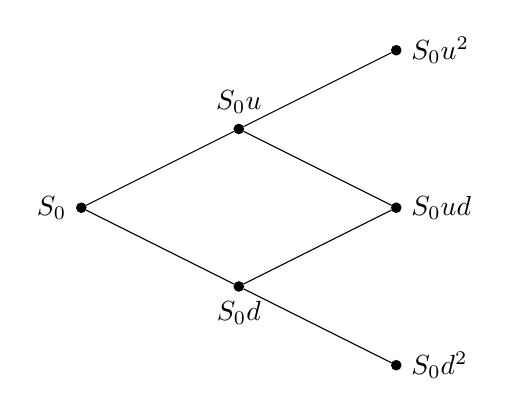
\begin{tikzpicture}[scale=2]
		% Nodes with dots
		\node[draw, fill=black, circle, inner sep=1.2pt, label=left:{$S_0$}] (S0) at (0,0) {};
		\node[draw, fill=black, circle, inner sep=1.2pt, label=above:{$S_0u$}] (Su) at (1,0.5) {};
		\node[draw, fill=black, circle, inner sep=1.2pt, label=below:{$S_0d$}] (Sd) at (1,-0.5) {};
		\node[draw, fill=black, circle, inner sep=1.2pt, label=right:{$S_0u^2$}] (Suu) at (2,1) {};
		\node[draw, fill=black, circle, inner sep=1.2pt, label=right:{$S_0ud$}] (Sud) at (2,0) {};
		\node[draw, fill=black, circle, inner sep=1.2pt, label=right:{$S_0d^2$}] (Sdd) at (2,-1) {};

		% Edges
		\draw[-] (S0) -- (Su);
		\draw[-] (S0) -- (Sd);
		\draw[-] (Su) -- (Suu);
		\draw[-] (Su) -- (Sud);
		\draw[-] (Sd) -- (Sud);
		\draw[-] (Sd) -- (Sdd);
	\end{tikzpicture}
	\caption{A two-step Binomial Tree}
	\label{fig:TwoStepBinomialTree}
\end{figure}

Alternatively we write this as

\[
	Z(t+1) \idef \frac{S(t+1)}{S(t)}, \quad t = 0, 1, \dots, T-1.
\]
We set up a probabilistic model by considering the $Z(t), t=1, \dots, T$ as random variables defined on probability spaces $(\tilde{\Omega}_t, \tilde{\F}_t, \tilde{\Prob}_t)$ with
\begin{align*}
	\tilde{\Omega}_t & = \tilde{\Omega} = \set{d, u},                                                                            \\
	\tilde{\F}_t     & = \tilde{\F} = \scP(\tilde{\Omega}) = \set{\emptyset, \set{d}, \set{u}, \tilde{\Omega}},                  \\
	\tilde{\Prob}_t  & = \tilde{\Prob} \text{ with } \tilde{\Prob}(\set{u}) = p, \ \tilde{\Prob}(\set{d}) = 1-p, \ p \in (0, 1).
\end{align*}
On these probability spaces we define
\[
	Z(t, u) = u \quad \text{and} \quad Z(t, d) = d, \quad t = 1, 2, \dots, T.
\]
Our aim, of course, is to define a probability space on which we can model the basic securities $(B, S)$. Since we can write the stock price as
\[
	S(t) = S(0) \prod_{\tau=1}^t Z(\tau), \quad t = 1, 2, \dots, T,
\]
the above definitions suggest using as the underlying probabilistic model of the financial market the \textit{product space} $(\Omega, \F, \Prob)$ (see e.g.\ [218] ch.\ 8), i.e.
\[
	\Omega = \tilde{\Omega}_1 \times \dots \times \tilde{\Omega}_T = \tilde{\Omega}^T = \set{d, u}^T,
\]
with each $\omega \in \Omega$ representing the successive values of $Z(t), t=1, 2, \dots, T$. Hence each $\omega \in \Omega$ is a $T$-tuple $\omega = (\tilde{\omega}_1, \dots, \tilde{\omega}_T)$ and $\tilde{\omega}_t \in \tilde{\Omega} = \set{d, u}$. For the $\sigma$-algebra we use $\F = \scP(\Omega)$ and the probability measure is given by
\[
	\Prob(\set{\omega}) = \tilde{\Prob}_1(\set{\omega_1}) \times \dots \times \tilde{\Prob}_T(\set{\omega_T}) = \tilde{\Prob}(\set{\omega_1}) \times \dots \times \tilde{\Prob}(\set{\omega_T}).
\]
The role of a product space is to model independent replication of a random experiment. The $Z(t)$ above are two-valued random variables, so can be thought of as tosses of a biased coin; we need to build a probability space on which we can model a succession of such independent tosses.

Now we redefine (with a slight abuse of notation) the $Z(t), t=1, \dots, T$ as random variables on $(\Omega, \F, \Prob)$ (as the $t$th projection)
\[
	Z(t, \omega) = Z(t, \omega_t).
\]
Observe that by this definition (and the above construction) $Z_1, \dots, Z_T$ are independent and identically distributed with
\[
	\Prob(Z(t) = u) = p = 1 - \Prob(Z(t) = d).
\]
To model the flow of information in the market we use the obvious filtration
\begin{align*}
	\F_0 & = \set{\emptyset, \Omega}                                &  & \text{(trivial $\sigma$-field)},           \\
	\F_t & = \sigma(Z(1), \dots, Z(t)) = \sigma(S(1), \dots, S(t)), &  &                                            \\
	\F_T & = \F = \scP(\Omega)                                      &  & \text{(class of all subsets of $\Omega$)}.
\end{align*}

This construction emphasises again that a multi-period model can be
viewed as a sequence of single-period models. Indeed, in the Cox-RossRubinstein case, we use identical and independent single-period models. As we will see in the sequel, this will make the construction of equivalent martingale measures relatively easy. Unfortunately, we can hardly defend the assumption of independent and identically distributed price movements at each time period
in practical applications.

\begin{xattention}
	We use this example to show how to construct the underlying probability space. Having done this in full once, we will from now on feel free to take for granted the existence of an appropriate probability space on which all relevant random variables are defined.
\end{xattention}

We now turn to the pricing of derivative assets in the Cox-Ross-Rubinstein market model. To do so we first have to discuss whether the Cox-Ross-Rubinstein model is arbitrage-free and complete.

Our first task is to find an equivalent martingale measure of the same class as $\Prob$, i.e.\ a probability measure $\bQ$ defined as a product measure via a measure $\tilde{\bQ}$ on $(\tilde{\Omega}, \tilde{\F})$ such that $\tilde{\bQ}(\set{u}) = q$ and $\tilde{\bQ}(\set{d}) = 1-q$. We call the set of all measures of that type $\scP$. We have:

\begin{prop}{Martingale Measure Existence}{MartingaleMeasureExistence}
	\begin{enumerate}[(i)]
		\item A martingale measure $\bQ \in \scP$ for the discounted stock price $\tilde{S}$ exists if and only if
		      \begin{equation}
			      d < 1+r < u.
			      \label{eq:CRRNoArb}
		      \end{equation}
		\item If \Cref{eq:CRRNoArb} holds true, then there is a unique such measure in $\scP$ characterised by
		      \begin{equation}
			      q = \frac{1+r-d}{u-d}.
		      \end{equation}
	\end{enumerate}
\end{prop}

\begin{proof}
	Since $S(t) = \tilde{S}(t)B(t) = \tilde{S}(t)(1+r)^t$, we have $Z(t+1) = S(t+1)/S(t) = (\tilde{S}(t+1)/\tilde{S}(t))(1+r)$. So, the discounted price $(\tilde{S}(t))$ is a $\bQ$-martingale if and only if for $t = 0, 1, \dots, T-1$
	\[
		\E^{\bQ}[\tilde{S}(t+1) \gvn \cF_t] = \tilde{S}(t) \iff \E^{\bQ}[(\tilde{S}(t+1)/\tilde{S}(t)) \gvn \cF_t] = 1 \iff \E^{\bQ}[Z(t+1) \gvn \cF_t] = 1+r.
	\]
	But $Z(1), \dots, Z(T)$ are mutually independent and hence $Z(t+1)$ is independent of $\cF_t = \sigma(Z(1), \dots, Z(t))$. So
	\[
		1+r = \E^{\bQ}(Z(t+1) \gvn \cF_t) = \E^{\bQ}(Z(t+1)) = uq + d(1-q)
	\]
	is a weighted average of $u$ and $d$; this can be $1+r$ if and only if $1+r \in [d, u]$. As $\bQ$ is to be \textit{equivalent} to $\Prob$ and $\Prob$ has no non-empty null sets, $r=d-1, u-1$ are excluded and \Cref{eq:CRRNoArb} is proved.

	To prove uniqueness and to find the value of $q$ we simply observe that under \Cref{eq:CRRNoArb}
	\[
		u \cdot q + d \cdot (1-q) = 1+r
	\]
	has a unique solution. Solving it for $q$ leads to the above formula.
\end{proof}

\begin{cor}{Arbitrage-Free Model}{arb_free}
	The Cox-Ross-Rubinstein model is arbitrage-free.
\end{cor}

\begin{proof}
	By \Cref{prop:MartingaleMeasureExistence} there exists an equivalent martingale measure and this is by the no-arbitrage theorem, \Cref{thm:NoArbitrage} enough to guarantee that the Cox-Ross-Rubinstein model is free of arbitrage.
\end{proof}

To answer the question of market completeness we have to examine the structure of equivalent martingale measures. We already know that there is a unique martingale measure in the class $\scP$, but can we find other equivalent martingale measures outside $\scP$? Examining the structure of the underlying measure space (product space) again we can show that every probability measure is a product measure, and hence all probability measures are of class $\scP$. Using this result we conclude the following:

\begin{prop}{CRR Model Completeness}{crr_complete}
	The Cox-Ross-Rubinstein model is complete.
\end{prop}

\begin{proof}
	Since by \Cref{prop:MartingaleMeasureExistence} the equivalent martingale measure is unique, the claim follows from the completeness theorem (\Cref{thm:CompletenessTheorem}).
\end{proof}

We translate the above measure-theoretic argument to economic language. Since every probability measure is a product measure uniqueness of the equivalent martingale measure on the product space is equivalent to uniqueness of the individual martingale measures on the component space. (Observe that this is true for general product space situations, it merely says that for independent random variables, the individual distributions determine the joint distribution.) We thus have the following result.

\begin{cor}{Multi-Period Completeness}{Multi-PeriodCompleteness}
	The multi-period model is complete if and only if every underlying single-period model is complete.
\end{cor}

We can now use the risk-neutral valuation formula to price every contingent claim in the Cox-Ross-Rubinstein model.

\begin{prop}{Arbitrage Price Process}{ArbitragePriceProcess}
	The arbitrage price process of a contingent claim $X$ in the Cox-Ross-Rubinstein model is given by
	\[
		\pi_X(t) = B(t)\E^* (X/B(T) \mid \F_t) \quad \forall t = 0, 1, \dots, T,
	\]
	where $\E^*$ is the expectation operator with respect to the unique equivalent martingale measure $\Prob^*$ characterised by $p^* = (1+r-d)/(u-d)$.
\end{prop}

\begin{cor}{European Call Valuation}{EuropeanCallValuation}
	Consider a European call option with expiry $T$ and strike price $K$ written on (one share of) the stock $S$. The arbitrage price process $C(t), t=0,1,\dots,T$ of the option is given by (set $\tau = T-t$)
	\begin{equation} \label{eq:EuropeanCallValuation}
		C(t) = (1+r)^{-\tau} \sum_{j=0}^{\tau} \bincof{\tau}{j} p^{*j}(1-p^*)^{\tau-j}(S(t)u^j d^{\tau-j} - K)^+.
	\end{equation}
\end{cor}

Since the Cox-Ross-Rubinstein model is complete we can find unique hedging strategies for replicating contingent claims. Recall that this means we can find a portfolio $\varphi(t) = (\varphi_0(t), \varphi_1(t))$, $\varphi$ predictable, such that the value process $V_\varphi(t) = \varphi_0(t)B(t) + \varphi_1(t)S(t)$ satisfies
\[
	\Pi_X(t) = V_\varphi(t), \quad \text{for all } t = 0, 1, \dots, T.
\]
Using the bond as num\'{e}raire we get the discounted equation
\[
	\tilde{\Pi}_X(t) = \tilde{V}_\varphi(t) = \varphi_0(t) + \varphi_1(t)\tilde{S}(t), \quad \text{for all } t = 0, 1, \dots, T.
\]
By the pricing formula, \Cref{prop:ArbitragePriceProcess}, we know the arbitrage price process and using the restriction of predictability of $\varphi$, this leads to a unique replicating portfolio process $\varphi$. We can compute this portfolio process at any point in time as follows. The equation $\tilde{\Pi}_X(t) = \varphi_0(t) + \varphi_1(t)\tilde{S}(t)$ has to be true for each $\omega = (\omega_1, \dots, \omega_t, \dots, \omega_T) \in \Omega$ and each $t = 1, \dots, T$ (observe that $\pi_X(0) = V_\varphi(0) = \varphi_0(1) + \varphi_1(1)S_1(0)$). Given such a $t$ we only can use information up to (and including) time $t-1$ to ensure that $\varphi$ is predictable. Therefore we know the coordinates $\omega_1, \dots, \omega_{t-1}$, but $\omega_t$ can only have one of the values $d$ or $u$. This leads to the following system of equations, which can be solved for $\varphi_0(t)$ and $\varphi_1(t)$ uniquely. With a slight abuse of notation we write $\tilde{\omega} = (\omega_1, \dots, \omega_{t-1})$, $\tilde{\omega}u = (\omega_1, \dots, \omega_{t-1}, u)$ and $\tilde{\omega}d = (\omega_1, \dots, \omega_{t-1}, d)$ (recall that since $S(t)$ and $\Pi_X(t)$ are $\F_t$-measurable they are constant on the corresponding partition $\scP_t$ of $\Omega$, which in our current setting is just given by the first $t$ coordinates of $\omega$, and the same argument applies for $\varphi$). Then
\begin{align*}
	\tilde{\Pi}_X(t, \tilde{\omega}u) & = \varphi_0(t, \tilde{\omega}) + \varphi_1(t, \tilde{\omega})\tilde{S}(t, \tilde{\omega}u), \\
	\tilde{\Pi}_X(t, \tilde{\omega}d) & = \varphi_0(t, \tilde{\omega}) + \varphi_1(t, \tilde{\omega})\tilde{S}(t, \tilde{\omega}d).
\end{align*}
The solution is given by
\begin{align*}
	\varphi_0(t, \tilde{\omega}) & = \frac{\tilde{S}(t, \tilde{\omega}u)\tilde{\Pi}_X(t, \tilde{\omega}d) - \tilde{S}(t, \tilde{\omega}d)\tilde{\Pi}_X(t, \tilde{\omega}u)}{\tilde{S}(t, \tilde{\omega}u) - \tilde{S}(t, \tilde{\omega}d)} \\
	                             & = \frac{u\tilde{\Pi}_X(t, \tilde{\omega}d) - d\tilde{\Pi}_X(t, \tilde{\omega}u)}{u-d},                                                                                                                  \\[8pt]
	\varphi_1(t, \tilde{\omega}) & = \frac{\tilde{\Pi}_X(t, \tilde{\omega}u) - \tilde{\Pi}_X(t, \tilde{\omega}d)}{\tilde{S}(t, \tilde{\omega}u) - \tilde{S}(t, \tilde{\omega}d)}                                                           \\
	                             & = \frac{\tilde{\Pi}_X(t, \tilde{\omega}u) - \tilde{\Pi}_X(t, \tilde{\omega}d)}{\tilde{S}(t-1, \tilde{\omega})(u-d)}.
\end{align*}
Observe that we only need to know $\tilde{\omega}$ to compute $\varphi(t)$, hence $\varphi$ is predictable. We make this rather abstract construction more transparent by constructing the hedge portfolio for the European call. We use the following notation. Write
\[
	C(t, x) \idef (1+r)^{-(T-t)} \sum_{j=0}^{T-t} \bincof{T-t}{j} p^{*j} (1-p^*)^{T-t-j} (x u^j d^{T-t-j} - K)^+.
\]
Then $C(t, x)$ is value of the call at time $t$ given that $S(t) = x$.

\begin{prop}{Perfect Hedging Strategy}{PerfectHedgingStrategy}
	The perfect hedging strategy $\varphi = (\varphi_0, \varphi_1)$ replicating the European call option with time of expiry $T$ and strike price $K$ is given by
	\begin{align*}
		\varphi_1(t) & = \frac{C(t, S(t-1)u) - C(t, S(t-1)d)}{S(t-1)(u-d)},    \\
		\varphi_0(t) & = \frac{uC(t, S(t-1)d) - dC(t, S(t-1)u)}{(1+r)^t(u-d)}.
	\end{align*}
\end{prop}

\begin{proof}
	$C(t, x)$ must be the value of the portfolio at time $t$ if the strategy $\varphi = (\varphi(t))$ replicates the claim:
	\[
		\varphi_0(t)(1+r)^t + \varphi_1(t)S(t) = C(t, S(t)).
	\]
	Now $S(t) = S(t-1)Z(t) = S(t-1)u$ or $S(t-1)d$, so:
	\begin{align*}
		\varphi_0(t)(1+r)^t + \varphi_1(t)S(t-1)u & = C(t, S(t-1)u), \\
		\varphi_0(t)(1+r)^t + \varphi_1(t)S(t-1)d & = C(t, S(t-1)d).
	\end{align*}
	Subtract:
	\[
		\varphi_1(t)S(t-1)(u-d) = C(t, S(t-1)u) - C(t, S(t-1)d).
	\]
	So $\varphi_1(t)$ in fact depends only on $S(t-1)$, thus yielding the predictability of $\varphi$, and
	\[
		\varphi_1(t) = \frac{C(t, S(t-1)u) - C(t, S(t-1)d)}{S(t-1)(u-d)}.
	\]
	Using any of the equations in the above system and solving for $\varphi_0(t)$ completes the proof.
\end{proof}

Notice that the numerator in the equation for $\varphi_1(t)$ is the difference of two values of $C(t, x)$, with the larger value of $x$ in the first term (recall $u > d$). When the payoff function $C(t, x)$ is an increasing function of $x$, as for the European call option considered here, this is non-negative. In this case, the Proposition gives $\varphi_1(t) \ge 0$: the replicating strategy does not involve short-selling. We record this as:

\begin{cor}{Monotone Payoff Hedging}{MonotonePayoffHedging}
	When the payoff function is a non-decreasing function of the asset price $S(t)$, the perfect-hedging strategy replicating the claim does not involve short-selling of the risky asset.
\end{cor}

If we do not use the pricing formula from \Cref{prop:ArbitragePriceProcess} (i.e.\ the information on the price process), but only the final values of the option (or more generally of a contingent claim) we are still able to compute the arbitrage price and to construct the hedging portfolio by backward induction. We outline this procedure for the European call starting with the last period $(T-1, T]$. We have to choose a replicating portfolio $\varphi(T) = (\varphi_0(T), \varphi_1(T))$ based on the information available at time $T-1$ (and so $\cF_{T-1}$-measurable). So for each $\omega \in \Omega$ the following equation has to hold:
\[
	C(T, \omega) = \varphi_0(T, \omega)B(T, \omega) + \varphi_1(T, \omega)S(T, \omega).
\]
Given the information $\cF_{T-1}$, we know all but the last coordinate of $\omega$, and this gives rise to two equations (with the same notation as above, $\tilde{\omega}$ denotes the first $T-1$ coordinates)
\begin{align*}
	C(T, \tilde{\omega}u) & = \varphi_0(T, \tilde{\omega})(1+r)^T + \varphi_1(T, \tilde{\omega})S(T, \tilde{\omega}u), \\
	C(T, \tilde{\omega}d) & = \varphi_0(T, \tilde{\omega})(1+r)^T + \varphi_1(T, \tilde{\omega})S(T, \tilde{\omega}d).
\end{align*}
Since we know the payoff structure of the call at time $T$, e.g.\ $C(T, \tilde{\omega}u) = (uS(T-1, \tilde{\omega}) - K)^{+}$ and $C(T, \tilde{\omega}d) = (dS(T-1, \tilde{\omega}) - K)^{+}$, we can solve the above system and obtain
\begin{align*}
	\varphi_1(T, \tilde{\omega}) & = \frac{(uS(T-1, \tilde{\omega}) - K)^{+} - (dS(T-1, \tilde{\omega}) - K)^{+}}{S(T-1, \tilde{\omega})(u - d)}, \\
	\varphi_0(T, \tilde{\omega}) & = \frac{u(dS(T-1, \tilde{\omega}) - K)^{+} - d(uS(T-1, \tilde{\omega}) - K)^{+}}{(1+r)(u - d)}.
\end{align*}
Using this portfolio one can compute the arbitrage price of the European call at time $T-1$ in state of the world $\tilde{\omega}$ as
\[
	C(T-1, \tilde{\omega}) = \varphi_0(T, \tilde{\omega})(1+r)^{T-1} + \varphi_1(T, \tilde{\omega})S(T-1, \tilde{\omega}).
\]
Now that the arbitrage prices at time $T-1$ are known, one can repeat the procedure to successively compute the prices at $T-2, \dots, 1, 0$.

The advantage of our risk-neutral pricing procedure over this approach is that we have a single formula for the price of the contingent claim at all times $t$, and don't have to resort to backward induction to compute a price at a special time $t$.

Using the pricing formula for the European call we see that the price process depends on the current stock price $S(t)$, the strike price $K$, the expiry date $T$, the interest rate $r$ and (hidden in $u, d$) the volatility of the stock price. We thus have the determining factors of the European call price explicit in \Cref{eq:EuropeanCallValuation} and can examine their effects explicitly. We use the notation $C(F)$ to mean that we consider the price $C$ of the call as a function of the factor $F$, keeping all others fixed.

\paragraph{Changes in Option Price Relative to the Underlying Stock Price.}

If the current stock price $S$ is changed by an amount $\Delta S$ we see that
\begin{align*}
	\Delta C & = C(S + \Delta S) - C(S)                                                                 \\
	         & = (1+r)^{-T} \sum_{j=0}^{T} \left( \bincof{T}{j} p^{*j}(1 - p^{*})^{T-j} \right.         \\
	         & \quad \left. \set*{((S + \Delta S)u^j d^{T-j} - K)^{+} - (Su^j d^{T-j} - K)^{+}} \right) \\
	         & \geq 0,
\end{align*}
since the function $(x - K)^{+}$ is increasing in $x$. Hence $C(S + \Delta S) \geq C(S)$ and the value of the option increases as the underlying stock price increases.

The quotient $\Delta C/\Delta S$ measures the change in the option price for an infinitesimal change in the stock price, keeping everything else fixed. If $\Delta S \to 0$ this quotient converges (under conditions of regularity) to $\partial C/\partial S$ and is therefore often referred to as the option's delta.

Looking at \Cref{prop:PerfectHedgingStrategy} we see the relation of the delta to the hedging portfolio for the option. The number of stocks to be held in the portfolio during period $(t - 1, t]$ is given by the difference quotient
\[
	\varphi_1(t) = \frac{C(t, S(t - 1)u) - C(t, S(t - 1)d)}{S(t - 1)u - S(t - 1)d}
\]
and this quotient is called the hedge ratio. This is an expression of the above type and we see that the number of stocks in the hedge portfolio is given approximately by the corresponding derivative, the option's delta.

\paragraph{Changes in Option Price Relative to the Strike Price $K$.}

Since the strike price $K$ is only present in the expression $(x - K)^{+}$ and this function is non-increasing in $K$, we immediately see that the options value is a non-increasing function of the strike price.

\Cref{eq:EuropeanCallValuation} can be used to discuss the other determining factors of the option price in a similar (although quite tedious) manner.

\subsection{Binomial Approximations}

Suppose we observe financial assets during a continuous time period $[0, T]$. To construct a stochastic model of the price processes of these assets (to e.g., value contingent claims) one basically has two choices

\begin{enumerate}[(i)]
	\item one could model the processes as continuous-time stochastic processes
	\item one could construct a sequence of discrete-time models in which the continuous-time price processes are approximated by discrete-time stochastic processes in a suitable sense.
\end{enumerate}

We describe the second approach now by examining the asymptotic properties of a sequence of Cox-Ross-Rubinstein models.

\subsubsection{Model Structure}

We assume that all random variables subsequently introduced are defined on a suitable probability space $(\Omega, \cF, \Pm)$. We want to model two assets, a riskless bond $B$ and a risky stock $S$, which we now observe in a continuous-time interval $[0, T]$. To transfer the continuous-time framework into a binomial structure we make the following adjustments. Looking at the $n$th Cox-Ross-Rubinstein model in our sequence, there is a prespecified number $k_n$ of trading dates. We set $\Delta_n = T/k_n$ and divide $[0, T]$ in $k_n$ subintervals of length $\Delta_n$, namely $I_j = [j\Delta_n, (j+1)\Delta_n]$, $j=0, \dots, k_n - 1$. We suppose that trading occurs only at the equidistant time points $t_{n,j} = j\Delta_n$, $j=0, \dots, k_n - 1$. We fix $r_n$ as the riskless interest rate over each interval $I_j$, and hence the bond process (in the $n$th model) is given by
\[
	B(t_{n,j}) = (1+r_n)^j, \quad j=0, \dots, k_n.
\]
In the continuous-time model we compound continuously with spot rate $r \geq 0$ and hence the bond price process $B(t)$ is given by $B(t) = \e^{rt}$. In order to approximate this process in the discrete-time framework, we choose $r_n$ such that
\begin{equation} \label{eq:RateApproximation}
	1 + r_n = \e^{r\Delta_n}.
\end{equation}
With this choice we have for any $j=0, \dots, k_n$ that $(1+r_n)^j = \exp(rj\Delta_n) = \exp(rt_{n,j})$. Thus we have approximated the bond process exactly at the time points of the discrete model.

Next we model the one-period returns $S(t_{n,j+1})/S(t_{n,j})$ of the stock by a family of random variables $Z_{n,i}; i=1, \dots, k_n$ taking values $\{d_n, u_n\}$ with
\[
	\Pm(Z_{n,i} = u_n) = p_n = 1 - \Pm(Z_{n,i} = d_n)
\]
for some $p_n \in (0, 1)$ (which we specify later). With these $Z_{n,j}$ we model the stock price process $S_n$ in the $n$th Cox-Ross-Rubinstein model as
\[
	S_n(t_{n,j}) = S_n(0) \prod_{i=1}^j Z_{n,i}, \quad j=0, 1, \dots, k_n.
\]
With the specification of the one-period returns we get a complete description of the discrete dynamics of the stock price process in each Cox-Ross-Rubinstein model. We call such a finite sequence $Z_n = (Z_{n,i})_{i=1}^{k_n}$ a lattice or tree. The parameters $u_n, d_n, p_n, k_n$ differ from lattice to lattice, but remain constant throughout a specific lattice. In the triangular array $(Z_{n,i}), i=1, \dots, k_n; n=1, 2, \dots$ we assume that the random variables are row-wise independent (but we allow dependence between rows). The approximation of a continuous-time setting by a sequence of lattices is called the lattice approach.

It is important to stress that for each $n$ we get a different discrete stock price process $S_n(t)$ and that in general these processes do not coincide on common time points (and are also different from the price process $S(t)$).

Turning back to a specific Cox-Ross-Rubinstein model, we now have a discrete-time bond and stock price process. We want arbitrage-free financial market models and therefore have to choose the parameters $u_n, d_n, p_n$ accordingly. An arbitrage-free financial market model is guaranteed by the existence of an equivalent martingale measure, and by \Cref{prop:MartingaleMeasureExistence}(i) the (necessary and) sufficient condition for that is
\[
	d_n < 1 + r_n < u_n.
\]
The risk-neutrality approach implies that the expected (under an equivalent martingale measure) one-period return must equal the one-period return of the riskless bond and hence we get (see \Cref{prop:MartingaleMeasureExistence}(ii))
\begin{equation} \label{eq:RiskNeutralProb}
	p_n = \frac{(1+r_n) - d_n}{u_n - d_n}.
\end{equation}
So the only parameters to choose freely in the model are $u_n$ and $d_n$. In the next sections we consider some special choices.

We now choose the parameters in the above lattice approach in a special way. Assuming the risk-free rate of interest $r$ is given, we have by \Cref{eq:RateApproximation}
\[
	1 + r_n = \e^{r\Delta_n},
\]
and the remaining degrees of freedom are resolved by choosing $u_n$ and $d_n$. We use the following choice:
\[
	u_n = \e^{\sigma\sqrt{\Delta_n}}, \quad d_n = u_n^{-1} = \e^{-\sigma\sqrt{\Delta_n}}.
\]
By condition \Cref{eq:RiskNeutralProb} the risk-neutral probabilities for the corresponding single-period models are given by
\[
	p_n^* = \frac{1 + r_n - d_n}{u_n - d_n}
	= \frac{\e^{r\Delta_n} - \e^{-\sigma\sqrt{\Delta_n}}}{\e^{\sigma\sqrt{\Delta_n}} - \e^{-\sigma\sqrt{\Delta_n}}}.
\]
We can now price contingent claims in each Cox-Ross-Rubinstein model using the expectation operator with respect to the (unique) equivalent martingale measure characterised by the probabilities $p_n^*$. In particular, we can compute the price $C(t)$ at time $t$ of a European call on the stock $S$ with strike $K$ and expiry $T$ by \Cref{eq:EuropeanCallValuation} of \Cref{prop:EuropeanCallValuation}. Let us reformulate this formula slightly. We define
\begin{equation}\label{eq:MinSteps}
	a_n = \min\{ j \in \N_0 \mid S(0)u_n^j d_n^{k_n-j} > K \}.
\end{equation}
Then we can rewrite the pricing formula \Cref{eq:EuropeanCallValuation} for $t=0$ in the setting of the $n$th Cox-Ross-Rubinstein model as
\begin{align*}
	C(0) & = (1+r_n)^{-k_n} \sum_{j=a_n}^{k_n} \binom{k_n}{j} p_n^{*\,j} (1-p_n^*)^{k_n-j} \bigl(S(0)u_n^j d_n^{k_n-j} - K\bigr)                     \\
	     & = S(0)\left[\sum_{j=a_n}^{k_n} \binom{k_n}{j}\left(\frac{p_n^* u_n}{1+r_n}\right)^j\left(\frac{(1-p_n^*)d_n}{1+r_n}\right)^{k_n-j}\right] \\
	     & \quad - K(1+r_n)^{-k_n}\left[\sum_{j=a_n}^{k_n} \binom{k_n}{j} p_n^{*\,j} (1-p_n^*)^{k_n-j}\right].
\end{align*}
Denoting the binomial cumulative distribution function with parameters $(n,p)$ as $B^{n,p}(\cdot)$ we see that the second bracketed expression is
\[
	\bar{B}^{k_n,p_n^*}(a_n) = 1 - B^{k_n,p_n^*}(a_n).
\]
Also the first bracketed expression is $\bar{B}^{k_n,\hat{p}_n}(a_n)$ with
\[
	\hat{p}_n = \frac{p_n^* u_n}{1+r_n}.
\]
That $\hat{p}_n$ is indeed a probability can be shown straightforwardly. Using this notation we have in the $n$th Cox-Ross-Rubinstein model for the price of a European call at time $t=0$ the following formula:
\begin{equation}\label{eq:CRRPricing}
	C_n(0) = S_n(0)\,\bar{B}^{k_n,\hat{p}_n}(a_n) - K(1+r_n)^{-k_n}\,\bar{B}^{k_n,p_n^*}(a_n).
\end{equation}
(We stress again that the underlying is $S_n(t)$, dependent on $n$, but $S_n(0)=S(0)$ for all $n$.) We now look at the limit of this expression.

\begin{prop}{Binomial Model Limit Relation}{LimitRelation}
	We have the following limit relation:
	\[
		\lim_{n\to\infty} C_n(0) = C_{BS}(0)
	\]
	with $C_{BS}(0)$ given by the Black-Scholes formula (we use $S = S(0)$ to ease the notation)
	\begin{equation}
		C_{BS}(0) = S N(d_1(S,T)) - K \e^{-rT} N(d_2(S,T)). \label{eq:BlackScholesFormula}
	\end{equation}
	The functions $d_1(s,t)$ and $d_2(s,t)$ are given by
	\begin{align*}
		d_1(s,t) & = \frac{\log(s/K) + (r + \frac{\sigma^2}{2})t}{\sigma\sqrt{t}},                            \\
		d_2(s,t) & = d_1(s,t) - \sigma\sqrt{t} = \frac{\log(s/K) + (r - \frac{\sigma^2}{2})t}{\sigma\sqrt{t}}
	\end{align*}
	and $N(.)$ is the standard normal cumulative distribution function.
\end{prop}

\begin{proof}
	Since $S_n(0) = S$ (say) all we have to do to prove the proposition is to show
	\begin{enumerate}[label=(\roman*)]
		\item $\displaystyle \lim_{n\to\infty} \xbar{B}^{k_n, \hat{p}_n}(a_n) = N(d_1(S,T))$,
		\item $\displaystyle \lim_{n\to\infty} \xbar{B}^{k_n, p_n^*}(a_n) = N(d_2(S,T))$.
	\end{enumerate}
	These statements involve the convergence of distribution functions.

	To show (i) we interpret
	\[
		\xbar{B}^{k_n, \hat{p}_n}(a_n) = \Prob(a_n \le Y_n \le k_n)
	\]
	with $(Y_n)$ a sequence of random variables distributed according to the binomial law with parameters $(k_n, \hat{p}_n)$. We normalise $Y_n$ to
	\[
		\tilde{Y}_n = \frac{Y_n - \E(Y_n)}{\sqrt{\Var(Y_n)}} = \frac{Y_n - k_n\hat{p}_n}{\sqrt{k_n\hat{p}_n(1-\hat{p}_n)}} = \frac{\sum_{j=1}^{k_n} (B_{j,n} - \hat{p}_n)}{\sqrt{k_n\hat{p}_n(1-\hat{p}_n)}},
	\]
	where $B_{j,n}$, $j=1,\dots,k_n$; $n=1,2,\dots$ are row-wise independent Bernoulli random variables with parameter $\hat{p}_n$. Now using the central limit theorem we know that for $\alpha_n \to \alpha$, $\beta_n \to \beta$ we have
	\[
		\lim_{n\to\infty} \Prob(\alpha_n \le \tilde{Y}_n \le \beta_n) = N(\beta) - N(\alpha).
	\]
	By definition we have
	\[
		\Prob(a_n \le Y_n \le k_n) = \Prob \left(\alpha_n \le \tilde{Y}_n \le \beta_n\right)
	\]
	with
	\[
		\alpha_n = \frac{a_n - k_n\hat{p}_n}{\sqrt{k_n\hat{p}_n(1-\hat{p}_n)}} \quad \text{and} \quad \beta_n = \frac{k_n(1-\hat{p}_n)}{\sqrt{k_n\hat{p}_n(1-\hat{p}_n)}}.
	\]
	Using the following limiting relations:
	\[
		\lim_{n\to\infty} \hat{p}_n = \frac{1}{2}, \quad \lim_{n\to\infty} k_n(1 - 2\hat{p}_n)\sqrt{\Delta_n} = -T \left(\frac{r}{\sigma} + \frac{\sigma}{2}\right),
	\]
	and the defining relation for $a_n$, \Cref{eq:MinSteps}, we get
	\begin{align*}
		\lim_{n\to\infty} \alpha_n & = \lim_{n\to\infty} \frac{\frac{\log(K/S) + k_n\sigma\sqrt{\Delta_n}}{2\sigma\sqrt{\Delta_n}} - k_n\hat{p}_n}{\sqrt{k_n\hat{p}_n(1-\hat{p}_n)}} \\
		                           & = \lim_{n\to\infty} \frac{\log(K/S) + \sigma k_n \sqrt{\Delta_n}(1 - 2\hat{p}_n)}{2\sigma \sqrt{k_n\Delta_n\hat{p}_n(1-\hat{p}_n)}}             \\
		                           & = \frac{\log(K/S) - (r + \frac{\sigma^2}{2})T}{\sigma\sqrt{T}} = -d_1(S,T).
	\end{align*}
	Furthermore we have
	\[
		\lim_{n\to\infty} \beta_n = \lim_{n\to\infty} \sqrt{k_n\hat{p}_n^{-1}(1 - \hat{p}_n)} = +\infty.
	\]
	So $N(\beta_n) \to 1, N(\alpha_n) \to N(-d_1) = 1 - N(d_1)$, completing the proof of (i).

	To prove (ii) we can argue in very much the same way and arrive at parameters $\alpha_n^*$ and $\beta_n^*$ with $\hat{p}_n$ replaced by $p_n^*$. Using the following limiting relations:
	\[
		\lim_{n\to\infty} p_n^* = \frac{1}{2}, \quad \lim_{n\to\infty} k_n(1 - 2p_n^*)\sqrt{\Delta_n} = T \left(\frac{\sigma}{2} - \frac{r}{\sigma}\right),
	\]
	we get
	\begin{align*}
		\lim_{n\to\infty} \alpha_n^* & = \lim_{n\to\infty} \frac{\log(K/S) + \sigma n \sqrt{\Delta_n}(1 - 2p_n^*)}{2\sigma \sqrt{n\Delta_n p_n^*(1 - p_n^*)}} \\
		                             & = \frac{\log(K/S) - (r - \frac{\sigma^2}{2})T}{\sigma\sqrt{T}} = -d_2(s, T).
	\end{align*}
	For the upper limit we get
	\[
		\lim_{n\to\infty} \beta_n^* = \lim_{n\to\infty} \sqrt{k_n (p_n^*)^{-1}(1 - p_n^*)} = +\infty,
	\]
	whence (ii) follows similarly.
\end{proof}

By the above proposition we have derived the classical Black-Scholes European call option valuation formula as an asymptotic limit of option prices in a sequence of Cox-Ross-Rubinstein type models with a special choice of parameters. We will therefore call these models discrete Black-Scholes models. Let us mention here that in the continuous-time Black-Scholes model the dynamics of the (stochastic) stock price process $S(t)$ are modelled by a geometric Brownian motion (or exponential Wiener process). The sample paths of this stochastic price process are almost all continuous and the probability law of $S(t)$ at any time $t$ is lognormal. In particular the time $T$ distribution of $\log\{S(T)/S(0)\}$ is $N(T\mu, T\sigma^2)$. Looking back at the construction of our sequence of Cox-Ross-Rubinstein models we see that

\begin{equation}
	\log\frac{S_n(T)}{S(0)} \;=\; \sum_{i=1}^{k_n} \log(Z_{n,i}).
\end{equation}

with \(\log(Z_{n,i})\) Bernoulli random variables with
\begin{equation}
	\Pm\!\big(\log(Z_{n,i})=\sigma\sqrt{\Delta_n}\big) \;=\; p_n
	\;=\; 1 - \Pm\!\big(\log(Z_{n,i})=-\sigma\sqrt{\Delta_n}\big).
\end{equation}

By the (triangular array version) of the central limit theorem we know that the
\(\log \frac{S_n(T)}{S(0)}\) properly normalised converges in distribution to a random
variable with standard normal distribution. Doing similar calculations as in the above
proposition we can compute the normalising constants and get
\begin{equation}
	\lim_{n\to\infty} \log\frac{S_n(T)}{S(0)} \;\sim\; \Nor\!\big(T(r-\sigma^2/2),\,T\sigma^2\big),
\end{equation}
i.e. \(S_n(T)/S(0)\) is in the limit lognormally distributed.

Using the terminology of weak convergence we can therefore say that the probability measures
\(\Pm^n\) induced by the distributions of \(S_n(T)/S(0)\) converge to the probability measure
\(\Q\) induced by \(\Nor\!\big(T(r-\sigma^2/2),\,T\sigma^2\big)\). Now the probability measures
\(\Pm^n\) are the risk-neutral equivalent probability measures in the \(n\)th Cox-Ross-Rubinstein
model, and we will show in Chapter 6 that in continuous-time market models, similarly to discrete-time
financial market modelling, contingent claims can be priced using risk-neutral equivalent martingale
measures. In particular we will show that in the above Black-Scholes market the (in this case unique)
equivalent martingale measure is given by \(\Q\).

\begin{prop}{Binomial Approximation Pricing Limit}{BinomialPricingLimit}
	Let $X$ be a contingent claim of the form $X = h(S(T))$ with $h$ a bounded, uniformly continuous real function. Denote by $\Pi_X^n$ resp.\ $\Pi_X$ the time $t = 0$ price of $X$ in the $n$th discrete-time resp.\ the continuous-time Black-Scholes market model. Then
	\[
		\lim_{n\to\infty} \Pi_X^n = \Pi_X.
	\]
\end{prop}
\begin{proof}
	Writing the pricing formula for the contingent claim using the expectation operator with respect to the risk-neutral probability measures, we have
	\[
		\Pi_X^n = \E_{\Prob^n}\!\big(h(S_n(T))\big) = \int h \,\di \Prob^n,
		\quad \text{resp.} \quad
		\Pi_X = \E_{\Q}\!\big(h(S(T))\big) = \int h \,\di \Q
	\]
	(since the $\sigma$-field at $t = 0$ is assumed to be trivial, we can use expectation instead of conditional expectation), and the portmanteau theorem gives the result.
\end{proof}
